\documentclass[12pt]{article}
\usepackage{listings}
\usepackage{xcolor}
\usepackage[margin=1in]{geometry}
\usepackage{amsmath,amsthm,amssymb}
\usepackage{graphicx}
\usepackage{epstopdf}
\DeclareGraphicsExtensions{.eps,.ps,.jpg,.bmp}
\lstset{
	numbers=left,
    framexleftmargin=10mm,
    frame=none,
    backgroundcolor=\color[RGB]{245,245,244},
	keywordstyle=\bf\color{blue},
	identifierstyle=\bf,
	numberstyle=\color[RGB]{0,192,192},
	commentstyle=\it\color[RGB]{0,96,96},
	stringstyle=\rmfamily\slshape\color[RGB]{128,0,0},
	showstringspaces=false
    }
% * <orcuslc@hotmail.com> 2016-03-02T15:13:09.253Z:
%
% ^.
 
\newcommand{\N}{\mathbb{N}}
\newcommand{\R}{\mathbb{R}}
\newcommand{\Z}{\mathbb{Z}}
\newcommand{\Q}{\mathbb{Q}}
 
\newenvironment{theorem}[2][Theorem]{\begin{trivlist}
\item[\hskip \labelsep {\bfseries #1}\hskip \labelsep {\bfseries #2.}]}{\end{trivlist}}
\newenvironment{lemma}[2][Lemma]{\begin{trivlist}
\item[\hskip \labelsep {\bfseries #1}\hskip \labelsep {\bfseries #2.}]}{\end{trivlist}}
\newenvironment{exercise}[2][Exercise]{\begin{trivlist}
\item[\hskip \labelsep {\bfseries #1}\hskip \labelsep {\bfseries #2.}]}{\end{trivlist}}
\newenvironment{problem}[2][Problem]{\begin{trivlist}
\item[\hskip \labelsep {\bfseries #1}\hskip \labelsep {\bfseries #2.}]}{\end{trivlist}}
\newenvironment{question}[2][Question]{\begin{trivlist}
\item[\hskip \labelsep {\bfseries #1}\hskip \labelsep {\bfseries #2.}]}{\end{trivlist}}
\newenvironment{corollary}[2][Corollary]{\begin{trivlist}
\item[\hskip \labelsep {\bfseries #1}\hskip \labelsep {\bfseries #2.}]}{\end{trivlist}}
 
\begin{document}
 
\title{Homework 2016-03-02}
\author{Chuan Lu\\ 
13300180056}
 
\maketitle
 
\begin{problem}{1}
\text{ }\\
When $x \to 0$, will the result of $f(x) = \frac{1 - cos(x)}{x ^{2}}$ be far from 0.5?
\end{problem}
\begin{proof}
The code is shown as follows.
\begin{lstlisting}[language={MATLAB}]
% homework1
% author: chuanlu
% 2016-03-02
format long
xx = 10 .^ [-1:-1:-16];
yy = (1 - cos(xx)) ./ (xx .^ 2);
semilogx(xx, yy);    
\end{lstlisting}
The result is shown as follows.
\begin{figure}[h!]
	\centering
    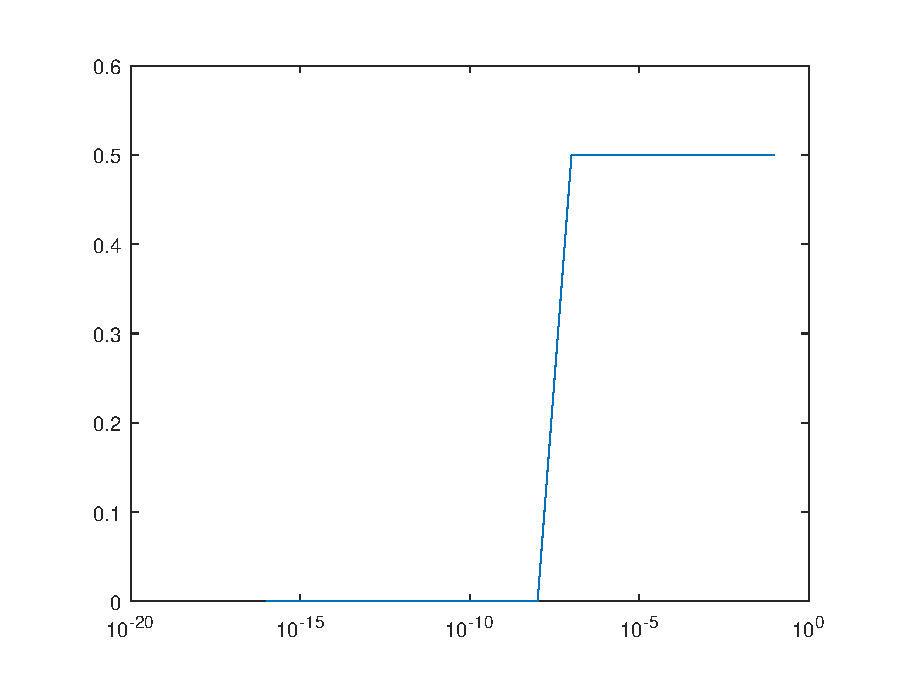
\includegraphics[width=11cm]{figure/problem1.eps}
    \caption{problem1}
    \label{problem1}
\end{figure}
\end{proof}

 
\begin{problem}{2}
\text{ }\\
Check the relationship of the conds of the two matrixs with their dims.
\end{problem}
\begin{proof}
The code is shown as follows, which means the statement is proved wrong.
\begin{lstlisting}[language={MATLAB}]
% make matrix
% author: chuanlu
% 2016-03-02
function [A] = make_matrix(op, n)
    
    if nargin < 1
        error('More args needed --make matrix');
    elseif nargin == 1
        op = 'A1';
    end
    
    if op == 'A1'
        c1 = zeros(1, n - 1);
        c1(2 : n - 1) = -3;
        c2 = zeros(1, n - 2) + 2;
        A = eye(n) + diag(c1, -1) + diag(c2, -2);
    elseif op == 'A2'
        c1 = zeros(1, n - 1);
        c1(2 : n - 1) = -3;
        c2 = zeros(1, n - 2) + 2;
        A = eye(n) + diag(c1, -1) + diag(c2, -2);
        A(1, n) = -1;
    else
        error('Operation Failed to Match A1 or A2');
    end
\end{lstlisting}

\begin{lstlisting}[language={MATLAB}]
% homework2.m
% author: chuanlu
% 2016-03-02

op1 = 'A1';
op2 = 'A2';
N = 100;
cond1 = zeros(1, N);
cond2 = zeros(1, N);
for n = 1 : N
    A1 = make_matrix(op1, n);
    A2 = make_matrix(op2, n);
    cond1(n) = cond(A1);
    cond2(n) = cond(A2);
end
n = [1:N];
figure(1);
semilogy(n, cond1, '*-');
figure(2);
plot(n, cond2, '*-');
%     disp('cond1:');
%     disp(cond1);
%     disp('cond2:');
%     disp(cond2);
\end{lstlisting}
The result is shown as follows.
\begin{figure}[htbp]
\begin{minipage}[t]{0.5\linewidth}
\centering
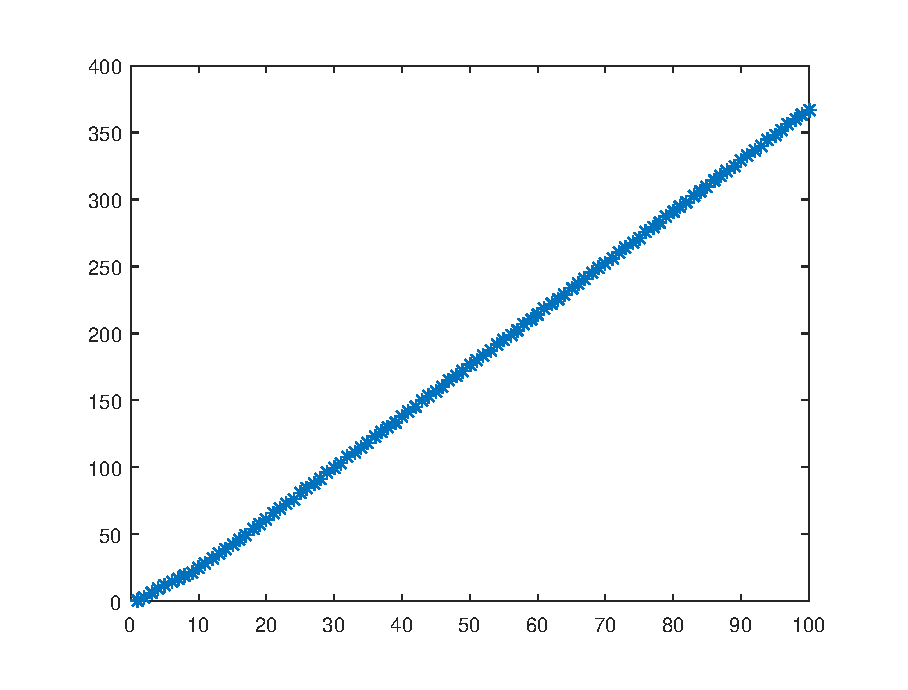
\includegraphics[width=0.8\textwidth]{figure/problem2-1.eps}
\caption{The relationship of cond($A_2$) with dim($A_2$), problem2-1}
\label{Problem2-1}
\end{minipage}
\begin{minipage}[t]{0.5\linewidth}
\centering
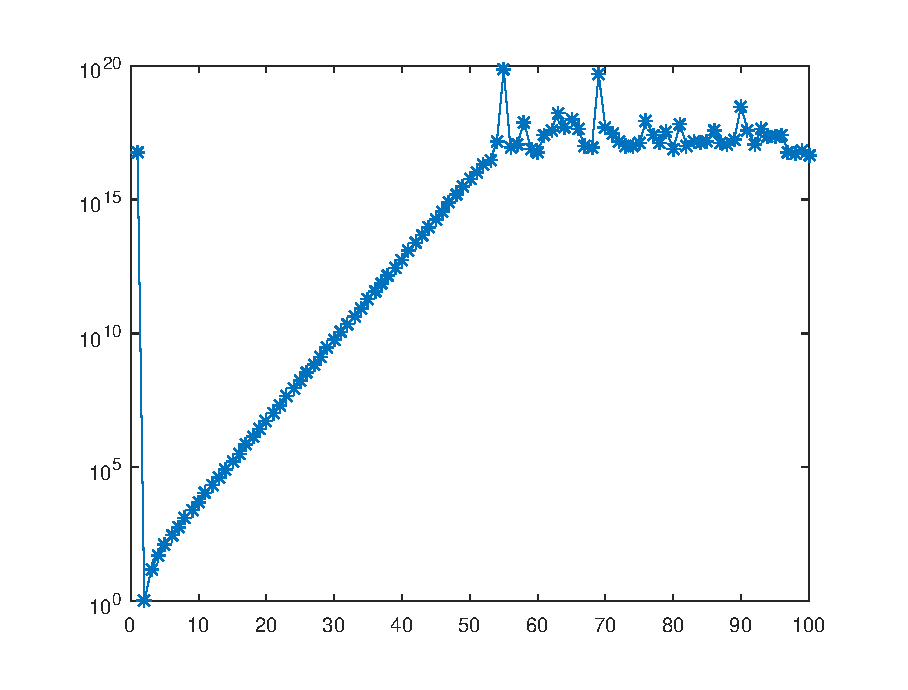
\includegraphics[width=0.8\textwidth]{figure/problem2-2.eps}
\caption{The relationship of cond($A_1$) with dim($A_1$), problem2-2}
\label{Problem2-2}
\end{minipage}
\end{figure}
\end{proof}

\begin{problem}{3}
\text{ }\\
Given $\Vert x_{n+2} - x_{n+1} \Vert$  $\leqslant$ $\alpha\Vert x_{n+1} - x_{n} \Vert$, then $\Vert x^{\star} - x_{n} \Vert$ $\leqslant$ $\frac{\alpha_{n}}{1-\alpha}\Vert x_{1} - x_{0}\Vert$.
\end{problem}
 
\begin{proof}
$\Vert x_{n} - x_{n - 1} \Vert\leqslant\alpha\Vert x_{n - 1} - x_{n - 2} \Vert\leqslant\dots\leqslant\alpha^{n-1}\Vert x_{1} - x_{0}\Vert$ \\
\par Hence, $\Vert x_{\star} - x_{n} \Vert\leqslant\Vert x_{n} - x_{n+1} \Vert+\Vert x_{n+1} - x_{n+2}\Vert + \dots\leqslant(\alpha^{n}+\alpha^{n+1}+\dots)\Vert x_{1} - x_{0}\Vert$ \\
\par$= \frac{\alpha^{n}}{1-\alpha}\Vert x_{1} - x_{0}\Vert$
\end{proof}

\end{document}
% \begin{problem}{4}
% \text{ }\\
% Suppose that $[a]$ is a unit in $\Z_{n}$ and $[b]$ is an element of $\Z_{n}$. Prove that the equation $[a]x = b$ has exactly one solution in $\Z_{n}$
% \end{problem}
 
% \begin{proof}

% \end{proof}

% \begin{problem}{5}
% \text{ }\\
% Suppose that $[a]$ and $[b]$ are both units in $\Z_{n}$.  Show that the product $[a] \cdot [b]$ is also a unit in $\Z_{n}.$ (Note that this confirms closure under multiplication in the group $U_{n})$.
% \end{problem}
 
% \begin{proof}

% \end{proof}

% \begin{problem}{6}
% \text{ }\\
% Which of the following are Groups? Which of the following are not groups, and why?\\

% \indent (1)  $G = \{{2, 4, 6, 8}\}$ in $\Z_{10}$.  Where $a \star b = ab$\\
% \indent (2)  $G = \Q^{\ast}$, where $a \star b = \frac{a}{b}$\\
% \indent (3) $G = \Z$, where $a \star b = a - b$\\
% \indent (4) $G = \{ {2^{x}\mid x \in \Q} \}$, where $a \star b = ab$\\
 
% \end{problem}
 
% \begin{proof}

% \end{proof}

% \begin{problem}{7}
% \text{ }\\
% Consider the set $Q =$ \{ $\pm$1, $\pm$i, $\pm$j, $\pm$k\} of the complex matrices as follows:\\
% \[
% 1=
%   \begin{bmatrix}
%     1 & 0\\
%     0 & 1\\
%   \end{bmatrix}
% \]

% \[
% i=
%   \begin{bmatrix}
%     i & 0\\
%     0 & $-$i\\
%   \end{bmatrix}
% \]

% \[
% j=
%   \begin{bmatrix}
%     0 & 1\\
%     $-$1 & 0\\
%   \end{bmatrix}
% \]

% \[
% k=
%   \begin{bmatrix}
%     0 & i\\
%     i & 0\\
%   \end{bmatrix}
% \]
% Show that $Q$ is a group under matrix multiplication by writing out its multiplicaiton table. (Note: $Q$ is called the quartenion group).
% \end{problem}
% \begin{proof}

% \end{proof}

% \end{document}
